\documentclass[a4paper,12pt]{article}
\usepackage{graphicx}
\usepackage{circuitikz}
\usepackage{amsmath}
\usepackage{booktabs}
\usepackage{hyperref}
\usepackage{caption}
\usepackage{float}
\usepackage{array}
\usepackage{tikz}
\title{\textbf{Assignment-08\\Design and Implementation of a Digital Synchronous UP/DOWN Counter}}
\author{EE24BTECH11021-ESHAN RAY\\ EE24BTECH11048-NITHIN.K}


\begin{document}

\maketitle

\section{Objective}
To design and implement a \textbf{digital up/down counter} that displays the number of people currently in the mess during peak lunch hours. The system will help students decide whether they can enter the mess based on the current occupancy. The maximum count is set to \textbf{99}.

\section{Components and Equipments}
\begin{table}[H]
	\centering
	\begin{tabular}{|c|c|c|}
		\hline
		\textbf{S.NO} & \textbf{Name of Material} & \textbf{Quantity} \\
		\hline
		1 & Dual J-K Flip-Flop(7476 ic) & 4 \\
		\hline
		2 & Triple 3-Input AND gate(7411 ic) & 12 \\
		\hline
		3 & Quad OR gate(7432 ic) & 4 \\
		\hline
		4 & Pushbutton & 2 \\
		\hline
		5 & Arduino/Power supply(5V) & 1 \\
		\hline
		6 & Resistors(300 $\Omega$) & 2 \\
		\hline
		7 & Resistors(1 K$\Omega$) & 2 \\
		\hline
		8 & 7-Segment Display & 2 \\
		\hline
		9 & 7-Segment Decoder(7447 ic) & 2 \\
		\hline
		10 & Breadboard & 5 \\
		\hline
		11 & Jumper wires & As much as required \\
		\hline
	\end{tabular}
\end{table}
\section{Procedutre}
\subsection{System Design and Working Principle}
\begin{enumerate}
    \item The IR sensors or ultrasonic sensors will be placed at the entry and exit points of the mess. But the same can be simulated using Buttons if the IR sensors are not available.
    \item When a person enters, the system increments the count (Up Counter).
    \item When a person leaves, the system decrements the count (Down Counter).
    \item The count is displayed on a 7-segment display.
    \item The Circuit is made up of only Logic gates and T flip-flops made from JK flip-flops.
    \item The outputs are then connected to a BCD decoder and then to a 7 Segment common anode display to show the count.
\end{enumerate}
\section{Circuit Design}
The T flip flop can be constructed from JK flip flop from the truth table shown below
\begin{table}[H]
\centering
\begin{tabular}{|c|c|c|c|c|}
\hline
	\textbf{Q} & \textbf{J} & \textbf{K} & \textbf{T} & \textbf{Q(next state)} \\
\hline
	0 & 0 & X & 0 & 0 \\
\hline
	0 & 1 & X & 1 & 1\\
\hline
	1 & X & 0 & 0 & 1 \\
\hline
	1 & X & 1 & 1 & 0 \\
\hline
\end{tabular}
\end{table}
From the table above we can conclude that \textbf{J = K = T}.
\newpage
\subsection{\textbf{State Transition Table For UP counter:}}
\begin{table}[H]
    \centering
    \begin{tabular}{c c c c | c c c c}
        \toprule
        \multicolumn{4}{c|}{Current State} & \multicolumn{4}{c}{Next State} \\
	    Q3 & Q2 & Q1 & Q0 & Q3 & Q2 & Q1 & Q0 \\
        \midrule
	    0 & 0 & 0 & 0 & 0 & 0 & 0 & 1 \\
	    0 & 0 & 0 & 1 & 0 & 0 & 1 & 0 \\
	    0 & 0 & 1 & 0 & 0 & 0 & 1 & 1 \\
	    0 & 0 & 1 & 1 & 0 & 1 & 0 & 0 \\
	    0 & 1 & 0 & 0 & 0 & 1 & 0 & 1 \\
	    0 & 1 & 0 & 1 & 0 & 1 & 1 & 0 \\
	    0 & 1 & 1 & 0 & 0 & 1 & 1 & 1 \\
	    0 & 1 & 1 & 1 & 1 & 0 & 0 & 0 \\
	    1 & 0 & 0 & 0 & 1 & 0 & 0 & 1 \\
	    1 & 0 & 0 & 1 & 0 & 0 & 0 & 0 \\
        \bottomrule
    \end{tabular}
\end{table}
\textbf{Truth Table For UP counter:}
\begin{table}[H]
        \begin{tabular}{|c|c|c|c|c|c|c|c|c|c|c|c|}
                \hline
		\textbf{Q3} & \textbf{Q2} & \textbf{Q1} & \textbf{Q0} & \textbf{T3} & \textbf{T2} & \textbf{T1} & \textbf{T0} & \textbf{Q3-next} & \textbf{Q2-next} & \textbf{Q1-next} & \textbf{Q0-next} \\
                \hline
		0 & 0 & 0 & 0 & 0 & 0 & 0 & 1 & 0 & 0 & 0 & 1 \\
                \hline
		0 & 0 & 0 & 1 & 0 & 0 & 1 & 1 & 0 & 0 & 1 & 0 \\
		\hline
		0 & 0 & 1 & 0 & 0 & 0 & 0 & 1 & 0 & 0 & 1 & 1 \\
		\hline
		0 & 0 & 1 & 1 & 0 & 1 & 1 & 1 & 0 & 1 & 0 & 0 \\
		\hline
		0 & 1 & 0 & 0 & 0 & 0 & 0 & 1 & 0 & 1 & 0 & 1 \\
		\hline
		0 & 1 & 0 & 1 & 0 & 0 & 1 & 1 & 0 & 1 & 1 & 0 \\
		\hline
		0 & 1 & 1 & 0 & 0 & 0 & 0 & 1 & 0 & 1 & 1 & 1 \\
		\hline
		0 & 1 & 1 & 1 & 1 & 1 & 1 & 1 & 1 & 0 & 0 & 0 \\
		\hline
		1 & 0 & 0 & 0 & 0 & 0 & 0 & 1 & 1 & 0 & 0 & 1 \\
		\hline
		1 & 0 & 0 & 1 & 1 & 0 & 0 & 1 & 0 & 0 & 0 & 0 \\
		\hline
		1 & 0 & 1 & 0 & X & X & X & X & X & X & X & X \\
		\hline
		1 & 0 & 1 & 1 & X & X & X & X & X & X & X & X \\
		\hline
		1 & 1 & 0 & 0 & X & X & X & X & X & X & X & X \\
		\hline
		1 & 1 & 0 & 1 & X & X & X & X & X & X & X & X \\
		\hline
		1 & 1 & 1 & 0 & X & X & X & X & X & X & X & X \\
		\hline
		1 & 1 & 1 & 1 & X & X & X & X & X & X & X & X \\
		\hline
        \end{tabular}
\end{table}
It is Obvious that $T_0$ is always 1 and for the remaining you have the below K-Maps
\begin{figure}[H]
\centering
\resizebox{0.9\textwidth}{!}{%
\begin{circuitikz}
\tikzstyle{every node}=[font=\normalsize]
\draw  (7.5,16) rectangle (11.5,12);
\draw [short] (7.5,15) -- (11.5,15);
\draw [short] (7.5,16) -- (6.75,16.75);
\node [font=\small] at (7.25,15.5) {00};
\node [font=\small] at (7.25,14.5) {01};
\node [font=\small] at (8,16.25) {00};
\node [font=\small] at (9,16.25) {01};
\node [font=\small] at (10,16.25) {11};
\node [font=\small] at (11,16.25) {10};
\draw [short] (8.5,16) -- (8.5,12);
\draw [short] (9.5,16) -- (9.5,12);
\draw [short] (10.5,16) -- (10.5,12);
\node [font=\small] at (6.5,16) {Q3};
\node [font=\small] at (7,16) {Q2};
\node [font=\small] at (7.75,16.75) {Q0};
\node [font=\small] at (7.25,16.75) {Q1};
\draw [short] (7.5,14) -- (11.5,14);
\draw [short] (7.5,13) -- (11.5,13);
\node [font=\small] at (7.25,13.5) {11};
\node [font=\small] at (7.25,12.5) {10};
\node [font=\normalsize] at (14,14) {$T_3 = Q_3Q_0 + Q_2Q_1Q_0$};
\node [font=\normalsize] at (10,14.5) {1};
\node [font=\normalsize] at (9,12.5) {1};
\node [font=\normalsize] at (11,12.5) {X};
\node [font=\normalsize] at (8,13.5) {X};
\node [font=\normalsize] at (9,13.5) {X};
\node [font=\normalsize] at (10,13.5) {X};
\node [font=\normalsize] at (11,13.5) {X};
\node [font=\normalsize] at (10,12.5) {X};
\draw [short] (9.75,13.25) -- (9.75,14.75);
\draw [short] (9.75,14.75) -- (10.25,14.75);
\draw [short] (10.25,14.75) -- (10.25,13.25);
\draw [short] (9.75,13.25) -- (10.25,13.25);
\draw [short] (8.75,12.25) -- (8.75,13.75);
\draw [short] (8.75,13.75) -- (10.25,13.75);
\draw [short] (8.75,12.25) -- (10.25,12.25);
\draw [short] (10.25,12.25) -- (10.25,13.75);
\draw  (7.5,10.25) rectangle (11.5,6.25);
\draw [short] (7.5,9.25) -- (11.5,9.25);
\draw [short] (7.5,10.25) -- (6.75,11);
\node [font=\small] at (7.25,9.75) {00};
\node [font=\small] at (7.25,8.75) {01};
\node [font=\small] at (8,10.5) {00};
\node [font=\small] at (9,10.5) {01};
\node [font=\small] at (10,10.5) {11};
\node [font=\small] at (11,10.5) {10};
\draw [short] (8.5,10.25) -- (8.5,6.25);
\draw [short] (9.5,10.25) -- (9.5,6.25);
\draw [short] (10.5,10.25) -- (10.5,6.25);
\node [font=\small] at (6.5,10.25) {Q3};
\node [font=\small] at (7,10.25) {Q2};
\node [font=\small] at (7.75,11) {Q0};
\node [font=\small] at (7.25,11) {Q1};
\draw [short] (7.5,8.25) -- (11.5,8.25);
\draw [short] (7.5,7.25) -- (11.5,7.25);
\node [font=\small] at (7.25,7.75) {11};
\node [font=\small] at (7.25,6.75) {10};
\node [font=\normalsize] at (14,8.25) {$T_2 = Q_1Q_0$};
\node [font=\normalsize] at (11,6.75) {X};
\node [font=\normalsize] at (8,7.75) {X};
\node [font=\normalsize] at (9,7.75) {X};
\node [font=\normalsize] at (10,7.75) {X};
\node [font=\normalsize] at (11,7.75) {X};
\node [font=\normalsize] at (10,6.75) {X};
\node [font=\normalsize] at (10,9.75) {1};
\node [font=\normalsize] at (10,8.75) {1};
\draw [short] (9.75,10) -- (9.75,6.5);
\draw [short] (9.75,10) -- (10.25,10);
\draw [short] (10.25,10) -- (10.25,6.5);
\draw [short] (9.75,6.5) -- (10.25,6.5);
\draw  (7.5,4.25) rectangle (11.5,0.25);
\draw [short] (7.5,3.25) -- (11.5,3.25);
\draw [short] (7.5,4.25) -- (6.75,5);
\node [font=\small] at (7.25,3.75) {00};
\node [font=\small] at (7.25,2.75) {01};
\node [font=\small] at (8,4.5) {00};
\node [font=\small] at (9,4.5) {01};
\node [font=\small] at (10,4.5) {11};
\node [font=\small] at (11,4.5) {10};
\draw [short] (8.5,4.25) -- (8.5,0.25);
\draw [short] (9.5,4.25) -- (9.5,0.25);
\draw [short] (10.5,4.25) -- (10.5,0.25);
\node [font=\small] at (6.5,4.25) {Q3};
\node [font=\small] at (7,4.25) {Q2};
\node [font=\small] at (7.75,5) {Q0};
\node [font=\small] at (7.25,5) {Q1};
\draw [short] (7.5,2.25) -- (11.5,2.25);
\draw [short] (7.5,1.25) -- (11.5,1.25);
\node [font=\small] at (7.25,1.75) {11};
\node [font=\small] at (7.25,0.75) {10};
\node [font=\normalsize] at (14,2.25) {$T_1 = \overline{Q_3}Q_0$};
\node [font=\normalsize] at (11,0.75) {X};
\node [font=\normalsize] at (8,1.75) {X};
\node [font=\normalsize] at (9,1.75) {X};
\node [font=\normalsize] at (10,1.75) {X};
\node [font=\normalsize] at (11,1.75) {X};
\node [font=\normalsize] at (10,0.75) {X};
\node [font=\normalsize] at (9,3.75) {$1$};
\node [font=\normalsize] at (10,3.75) {$1$};
\node [font=\normalsize] at (9,2.75) {$1$};
\node [font=\normalsize] at (10,2.75) {$1$};
\draw [short] (8.75,4) -- (8.75,2.5);
\draw [short] (8.75,4) -- (10.25,4);
\draw [short] (8.75,2.5) -- (10.25,2.5);
\draw [short] (10.25,4) -- (10.25,2.5);
\end{circuitikz}
}%
\end{figure}

\subsection{\textbf{State Transition Table For DOWN counter:}}
\begin{table}[H]
    \centering
    \begin{tabular}{c c c c | c c c c}
        \toprule
        \multicolumn{4}{c|}{Current State} & \multicolumn{4}{c}{Next State} \\
	    Q3 & Q2 & Q1 & Q0 & Q3 & Q2 & Q1 & Q0 \\
        \midrule
	    1 & 0 & 0 & 1 & 1 & 0 & 0 & 0 \\
	    1 & 0 & 0 & 0 & 0 & 1 & 1 & 1 \\
	    0 & 1 & 1 & 1 & 0 & 1 & 1 & 0 \\
	    0 & 1 & 1 & 0 & 0 & 1 & 0 & 1 \\
	    0 & 1 & 0 & 1 & 0 & 1 & 0 & 0 \\
	    0 & 1 & 0 & 0 & 0 & 0 & 1 & 1 \\
	    0 & 0 & 1 & 1 & 0 & 0 & 1 & 0 \\
	    0 & 0 & 1 & 0 & 0 & 0 & 0 & 1 \\
	    0 & 0 & 0 & 1 & 0 & 0 & 0 & 0 \\
	    0 & 0 & 0 & 0 & 1 & 0 & 0 & 1 \\
        \bottomrule
    \end{tabular}
\end{table}
\textbf{Truth Table For DOWN counter:}
\begin{table}[H]
        \begin{tabular}{|c|c|c|c|c|c|c|c|c|c|c|c|}
                \hline
		\textbf{Q3} & \textbf{Q2} & \textbf{Q1} & \textbf{Q0} & \textbf{T3} & \textbf{T2} & \textbf{T1} & \textbf{T0} & \textbf{Q3-next} & \textbf{Q2-next} & \textbf{Q1-next} & \textbf{Q0-next} \\
                \hline
                1 & 1 & 1 & 1 & X & X & X & X & X & X & X & X \\
                \hline
                1 & 1 & 1 & 0 & X & X & X & X & X & X & X & X \\
                \hline
                1 & 1 & 0 & 1 & X & X & X & X & X & X & X & X \\
                \hline
                1 & 1 & 0 & 0 & X & X & X & X & X & X & X & X \\
                \hline
                1 & 0 & 1 & 1 & X & X & X & X & X & X & X & X \\
                \hline
                1 & 0 & 1 & 0 & X & X & X & X & X & X & X & X \\
                \hline
		1 & 0 & 0 & 1 & 0 & 0 & 0 & 1 & 1 & 0 & 0 & 0 \\
                \hline
		1 & 0 & 0 & 0 & 1 & 1 & 1 & 1 & 0 & 1 & 1 & 1 \\
		\hline
		0 & 1 & 1 & 1 & 0 & 0 & 0 & 1 & 0 & 1 & 1 & 0 \\
		\hline
		0 & 1 & 1 & 0 & 0 & 0 & 1 & 1 & 0 & 1 & 0 & 1 \\
		\hline
		0 & 1 & 0 & 1 & 0 & 0 & 0 & 1 & 0 & 1 & 0 & 0 \\
		\hline
		0 & 1 & 0 & 0 & 0 & 1 & 1 & 1 & 0 & 0 & 1 & 1 \\
		\hline
		0 & 0 & 1 & 1 & 0 & 0 & 0 & 1 & 0 & 0 & 1 & 0 \\
		\hline
		0 & 0 & 1 & 0 & 0 & 0 & 1 & 1 & 0 & 0 & 0 & 1 \\
		\hline
		0 & 0 & 0 & 1 & 0 & 0 & 0 & 1 & 0 & 0 & 0 & 0 \\
		\hline
		0 & 0 & 0 & 0 & 1 & 0 & 0 & 1 & 1 & 0 & 0 & 1 \\
		\hline
        \end{tabular}
\end{table}
It is Obvious that $T_0$ is always 1 and for the remaining you have the below K-Maps
\begin{figure}[H]
\centering
\resizebox{1\textwidth}{!}{%
\begin{circuitikz}
\tikzstyle{every node}=[font=\normalsize]
\draw  (7.5,16) rectangle (11.5,12);
\draw [short] (7.5,15) -- (11.5,15);
\draw [short] (7.5,16) -- (6.75,16.75);
\node [font=\small] at (7.25,15.5) {00};
\node [font=\small] at (7.25,14.5) {01};
\node [font=\small] at (8,16.25) {00};
\node [font=\small] at (9,16.25) {01};
\node [font=\small] at (10,16.25) {11};
\node [font=\small] at (11,16.25) {10};
\draw [short] (8.5,16) -- (8.5,12);
\draw [short] (9.5,16) -- (9.5,12);
\draw [short] (10.5,16) -- (10.5,12);
\node [font=\small] at (6.5,16) {Q3};
\node [font=\small] at (7,16) {Q2};
\node [font=\small] at (7.75,16.75) {Q0};
\node [font=\small] at (7.25,16.75) {Q1};
\draw [short] (7.5,14) -- (11.5,14);
\draw [short] (7.5,13) -- (11.5,13);
\node [font=\small] at (7.25,13.5) {11};
\node [font=\small] at (7.25,12.5) {10};
\node [font=\normalsize] at (15,14) {$T_3 = \overline{Q_2}T, \,T = \overline{Q_1}\,\overline{Q_0}$};
\node [font=\normalsize] at (11,12.5) {X};
\node [font=\normalsize] at (8,13.5) {X};
\node [font=\normalsize] at (9,13.5) {X};
\node [font=\normalsize] at (10,13.5) {X};
\node [font=\normalsize] at (11,13.5) {X};
\node [font=\normalsize] at (10,12.5) {X};
\draw  (7.5,10.25) rectangle (11.5,6.25);
\draw [short] (7.5,9.25) -- (11.5,9.25);
\draw [short] (7.5,10.25) -- (6.75,11);
\node [font=\small] at (7.25,9.75) {00};
\node [font=\small] at (7.25,8.75) {01};
\node [font=\small] at (8,10.5) {00};
\node [font=\small] at (9,10.5) {01};
\node [font=\small] at (10,10.5) {11};
\node [font=\small] at (11,10.5) {10};
\draw [short] (8.5,10.25) -- (8.5,6.25);
\draw [short] (9.5,10.25) -- (9.5,6.25);
\draw [short] (10.5,10.25) -- (10.5,6.25);
\node [font=\small] at (6.5,10.25) {Q3};
\node [font=\small] at (7,10.25) {Q2};
\node [font=\small] at (7.75,11) {Q0};
\node [font=\small] at (7.25,11) {Q1};
\draw [short] (7.5,8.25) -- (11.5,8.25);
\draw [short] (7.5,7.25) -- (11.5,7.25);
\node [font=\small] at (7.25,7.75) {11};
\node [font=\small] at (7.25,6.75) {10};
\node [font=\normalsize] at (15.25,8.25) {$T_2 = (Q_2+Q_3)T,\, T = \overline{Q_1}\,\overline{Q_0}$};
\node [font=\normalsize] at (11,6.75) {X};
\node [font=\normalsize] at (8,7.75) {X};
\node [font=\normalsize] at (9,7.75) {X};
\node [font=\normalsize] at (10,7.75) {X};
\node [font=\normalsize] at (11,7.75) {X};
\node [font=\normalsize] at (10,6.75) {X};
\draw  (7.5,4.25) rectangle (11.5,0.25);
\draw [short] (7.5,3.25) -- (11.5,3.25);
\draw [short] (7.5,4.25) -- (6.75,5);
\node [font=\small] at (7.25,3.75) {00};
\node [font=\small] at (7.25,2.75) {01};
\node [font=\small] at (8,4.5) {00};
\node [font=\small] at (9,4.5) {01};
\node [font=\small] at (10,4.5) {11};
\node [font=\small] at (11,4.5) {10};
\draw [short] (8.5,4.25) -- (8.5,0.25);
\draw [short] (9.5,4.25) -- (9.5,0.25);
\draw [short] (10.5,4.25) -- (10.5,0.25);
\node [font=\small] at (6.5,4.25) {Q3};
\node [font=\small] at (7,4.25) {Q2};
\node [font=\small] at (7.75,5) {Q0};
\node [font=\small] at (7.25,5) {Q1};
\draw [short] (7.5,2.25) -- (11.5,2.25);
\draw [short] (7.5,1.25) -- (11.5,1.25);
\node [font=\small] at (7.25,1.75) {11};
\node [font=\small] at (7.25,0.75) {10};
\node [font=\normalsize] at (14,2.25) {$T_1 = Q_1\overline{Q_0}+T_2$};
\node [font=\normalsize] at (11,0.75) {X};
\node [font=\normalsize] at (8,1.75) {X};
\node [font=\normalsize] at (9,1.75) {X};
\node [font=\normalsize] at (10,1.75) {X};
\node [font=\normalsize] at (11,1.75) {X};
\node [font=\normalsize] at (10,0.75) {X};
\node [font=\normalsize] at (8,12.5) {1};
\node [font=\normalsize] at (8,15.5) {1};
\draw [short] (7.75,16.25) -- (7.75,15.25);
\draw [short] (7.75,15.25) -- (8.25,15.25);
\draw [short] (8.25,15.25) -- (8.25,16.25);
\draw [short] (7.75,11.75) -- (7.75,12.75);
\draw [short] (7.75,12.75) -- (8.25,12.75);
\draw [short] (8.25,12.75) -- (8.25,11.75);
\node [font=\normalsize] at (8,6.75) {$1$};
\node [font=\normalsize] at (8,8.75) {$1$};
\draw [short] (7.75,9) -- (7.75,7.5);
\draw [short] (8.25,9) -- (8.25,7.5);
\draw [short] (7.75,9) -- (8.25,9);
\draw [short] (7.75,7.5) -- (8.25,7.5);
\draw [short] (7.75,8) -- (7.75,6.5);
\draw [short] (7.75,6.5) -- (8.25,6.5);
\draw [short] (8.25,6.5) -- (8.25,8);
\draw [short] (8.25,8) -- (7.75,8);
\node [font=\normalsize] at (8,0.75) {$1$};
\node [font=\normalsize] at (11,2.75) {$1$};
\node [font=\normalsize] at (8,2.75) {$1$};
\node [font=\normalsize] at (11,3.75) {$1$};
\draw [short] (10.75,4) -- (10.75,0.5);
\draw [short] (10.75,0.5) -- (11.25,0.5);
\draw [short] (11.25,0.5) -- (11.25,4);
\draw [short] (10.75,4) -- (11.25,4);
\draw [short] (7.75,3) -- (7.75,1.5);
\draw [short] (7.75,3) -- (8.25,3);
\draw [short] (8.25,3) -- (8.25,1.5);
\draw [short] (7.75,1.5) -- (8.25,1.5);
\draw [short] (7.75,2) -- (7.75,0.5);
\draw [short] (7.75,0.5) -- (8.25,0.5);
\draw [short] (8.25,0.5) -- (8.25,2);
\draw [short] (8.25,2) -- (7.75,2);
\end{circuitikz}
}%
\end{figure}
\subsection{\textbf{Circuit Diagram}}
\textbf{The figures below are taken from Tinkercad simulated by us.}
\begin{figure}[H]
\centering
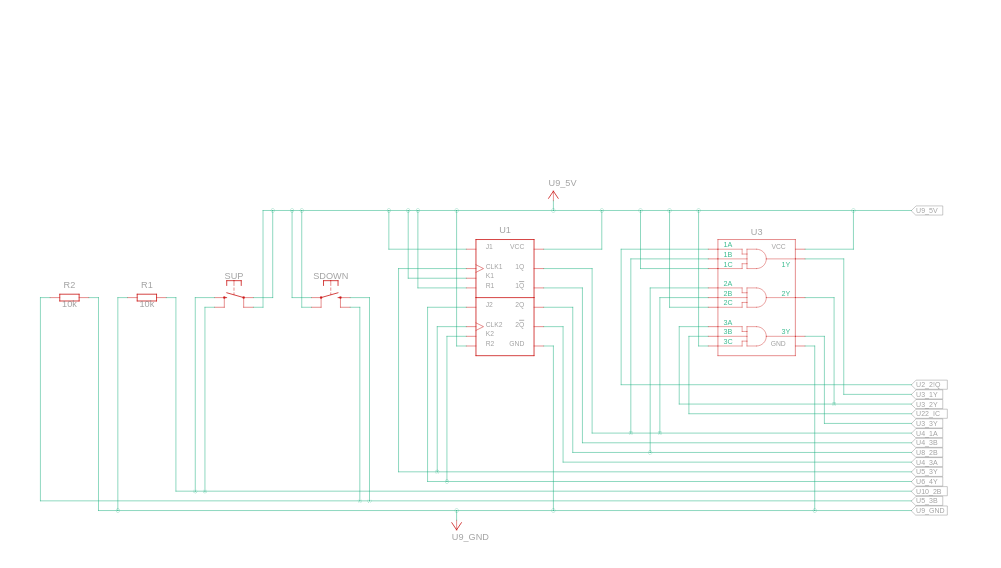
\includegraphics[width=1\textwidth]{figs/c1.png}
\caption{}
\end{figure}
\begin{figure}[H]
\centering    
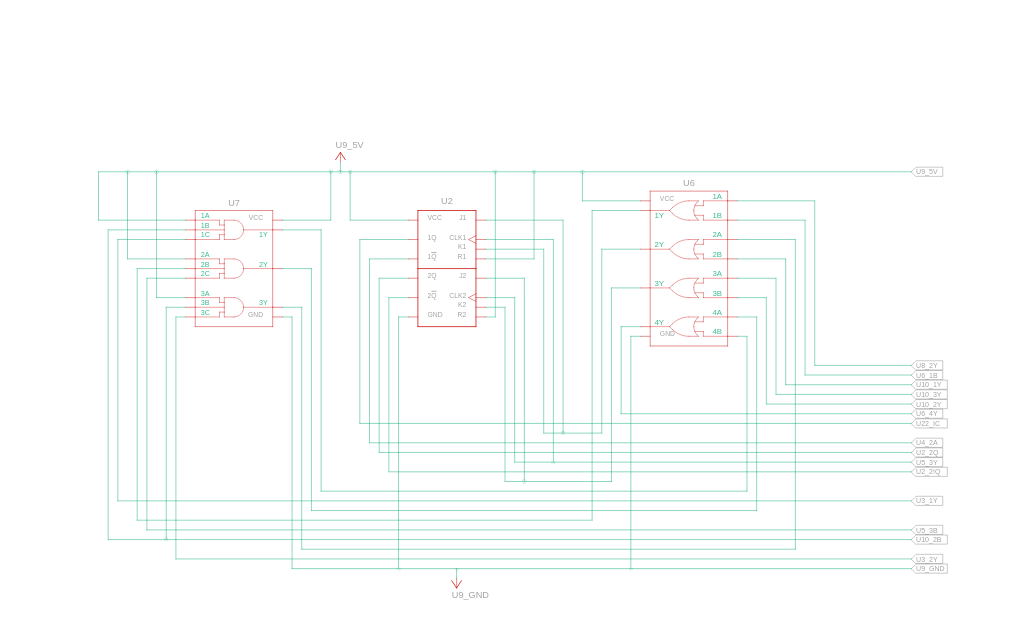
\includegraphics[width=1\textwidth]{figs/c2.png} 
\caption{}
\end{figure}
\begin{figure}[H]
\centering    
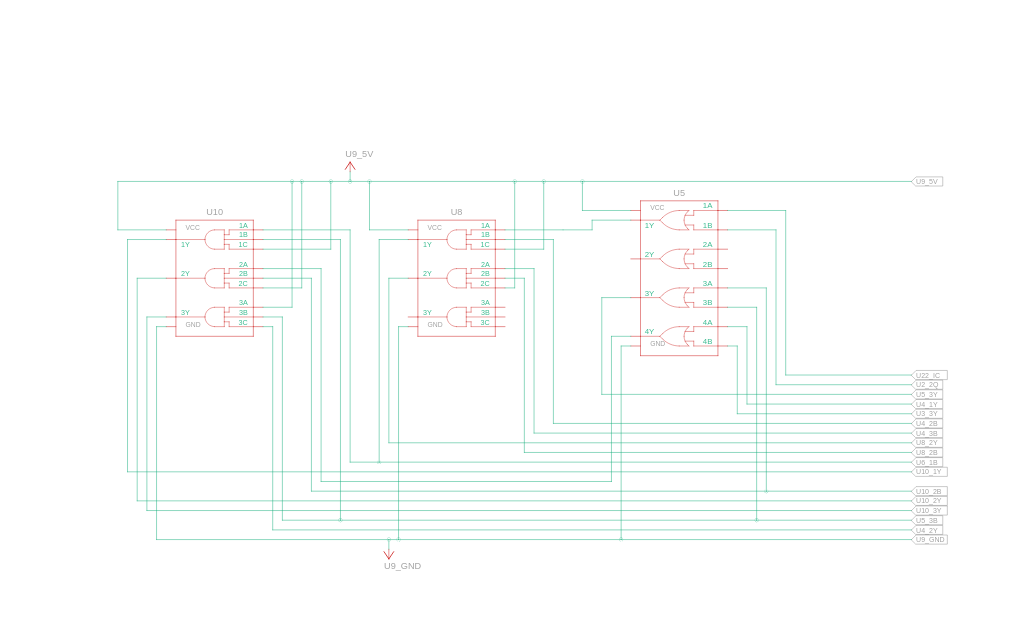
\includegraphics[width=1\textwidth]{figs/c3.png}
\caption{}
\end{figure}
\begin{figure}[H]
\centering    
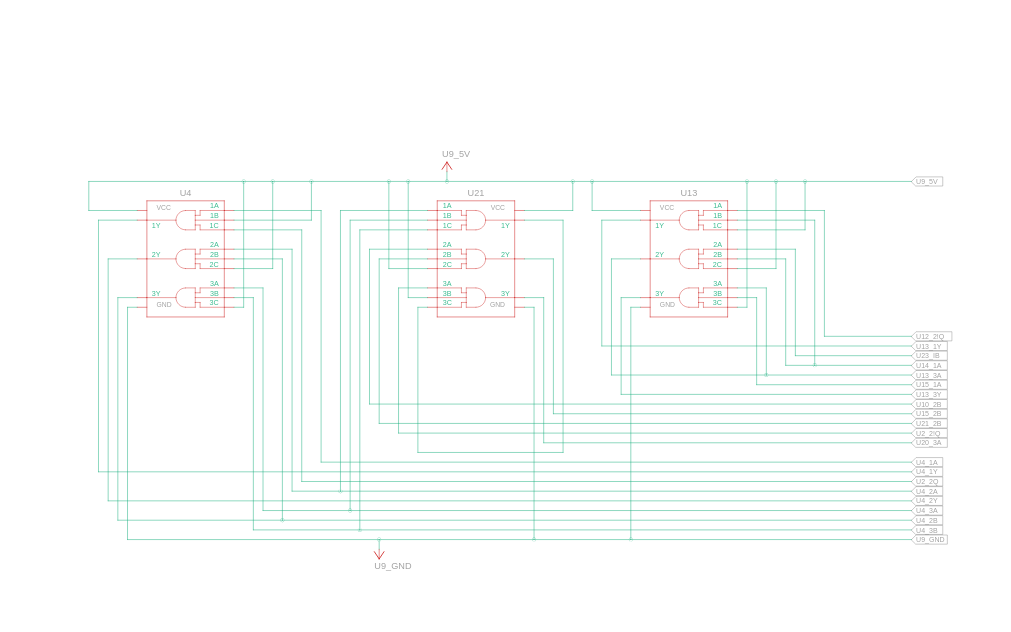
\includegraphics[width=1\textwidth]{figs/c4.png}
\caption{}
\end{figure}
\begin{figure}[H]
\centering    
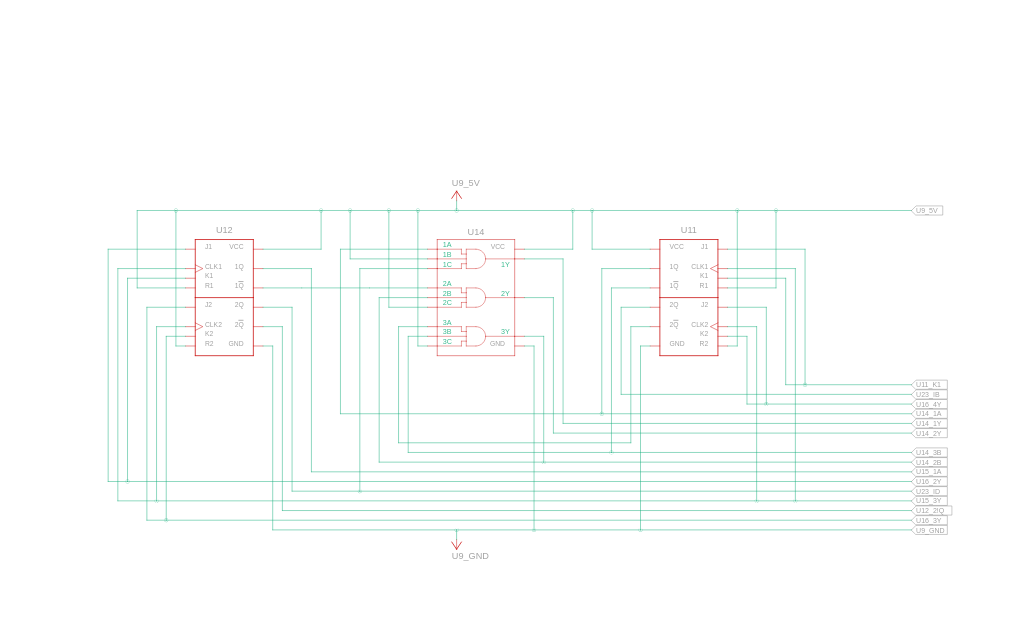
\includegraphics[width=1\textwidth]{figs/c5.png}
\caption{}
\end{figure}
\begin{figure}[H]
\centering    
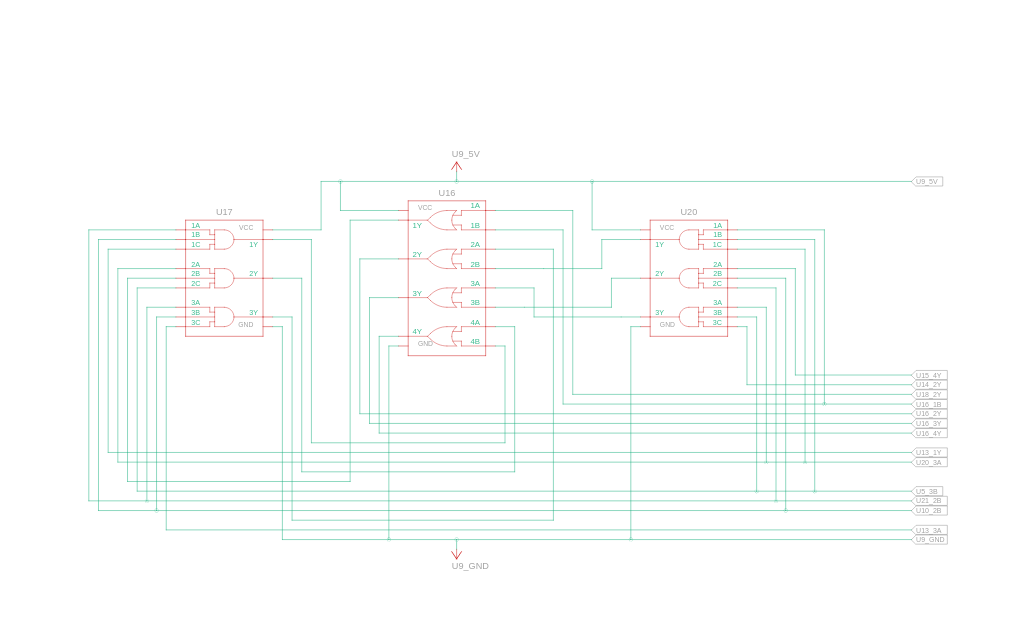
\includegraphics[width=1\textwidth]{figs/c6.png}
\caption{}
\end{figure}
\begin{figure}[H]
\centering    
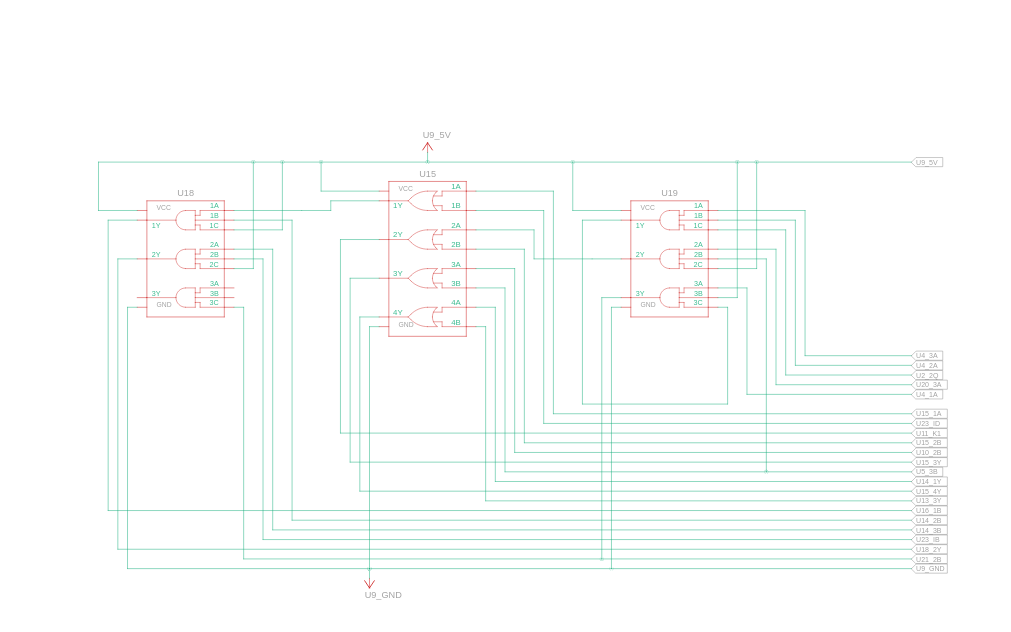
\includegraphics[width=1\textwidth]{figs/c7.png}
\caption{}
\end{figure}
\begin{figure}[H]
\centering    
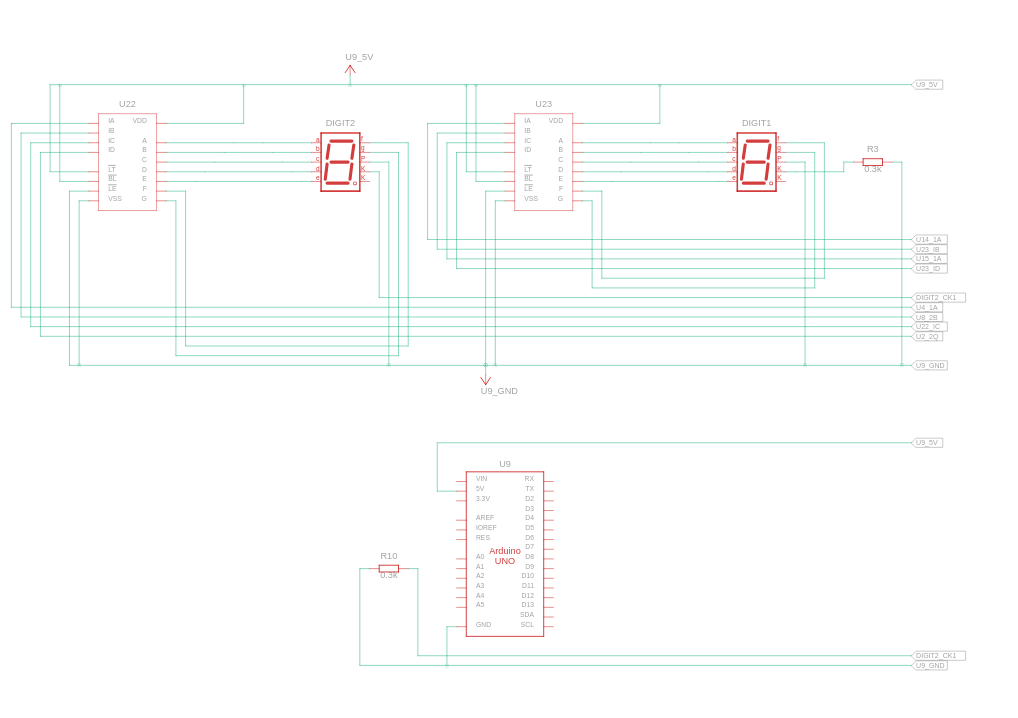
\includegraphics[width=1\textwidth]{figs/c8.png}
\caption{} 
\end{figure}
\begin{figure}[H]
\centering    
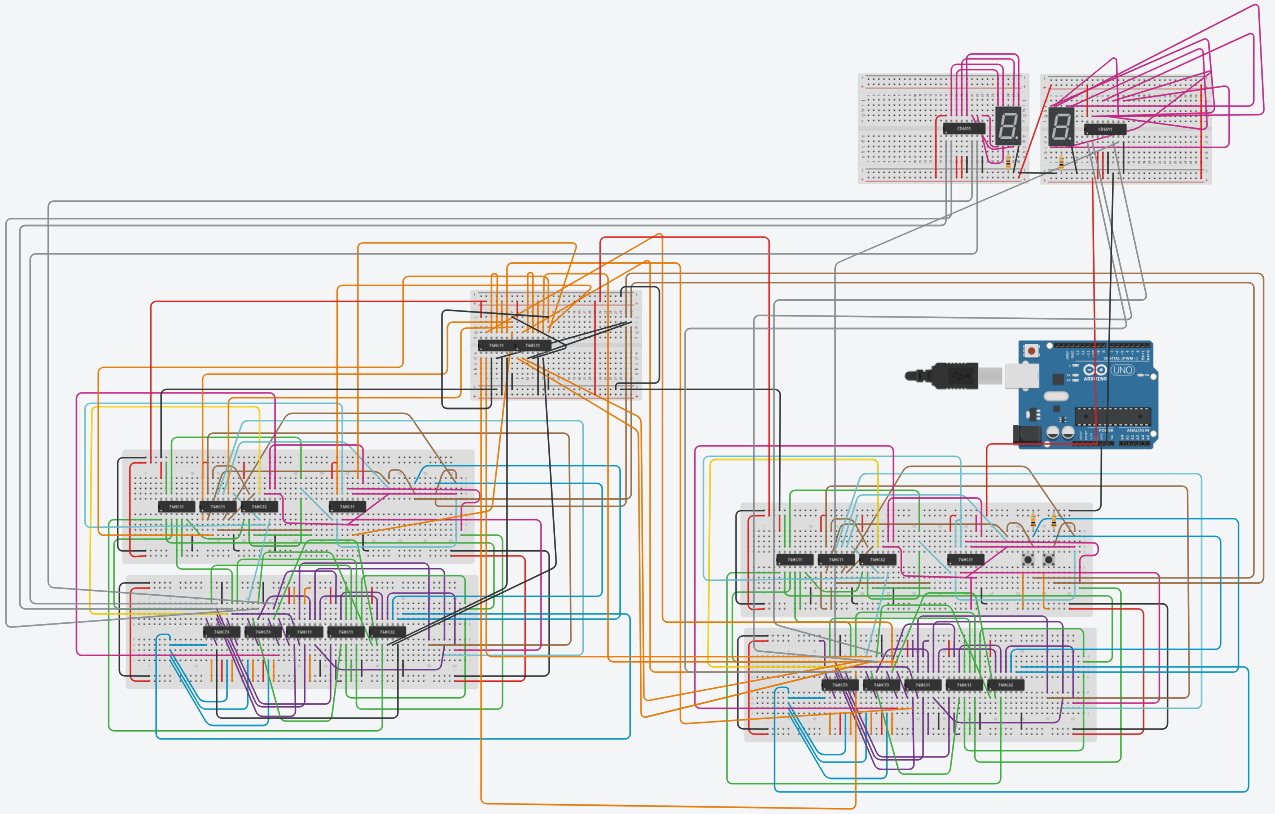
\includegraphics[width=1\textwidth]{figs/Circuit.png}
	\caption*{Circuit Figure In Simulation}
\end{figure}
\begin{figure}[H]
\centering
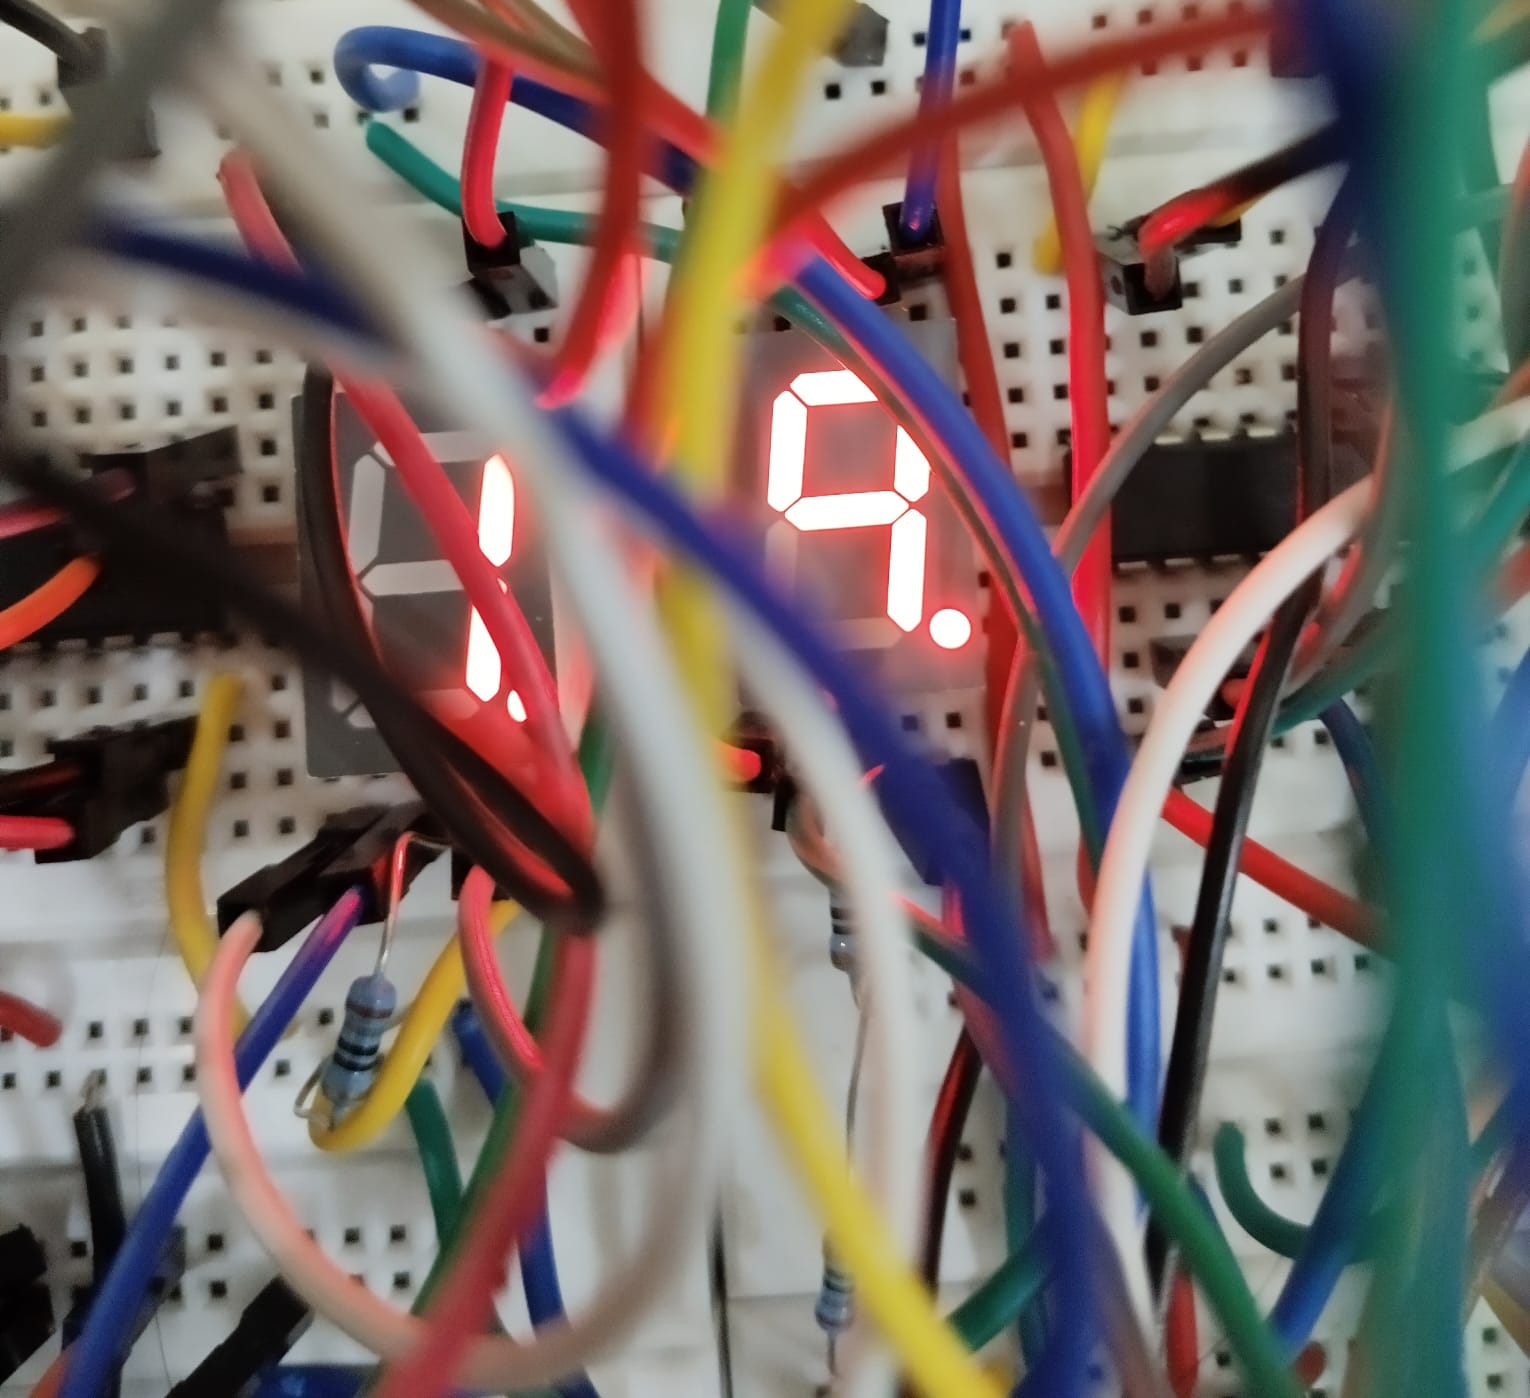
\includegraphics[width=0.6\textwidth]{figs/r_19.jpeg}
	\caption*{Circuit Displaying 19}
\end{figure}
\begin{figure}[H]
\centering
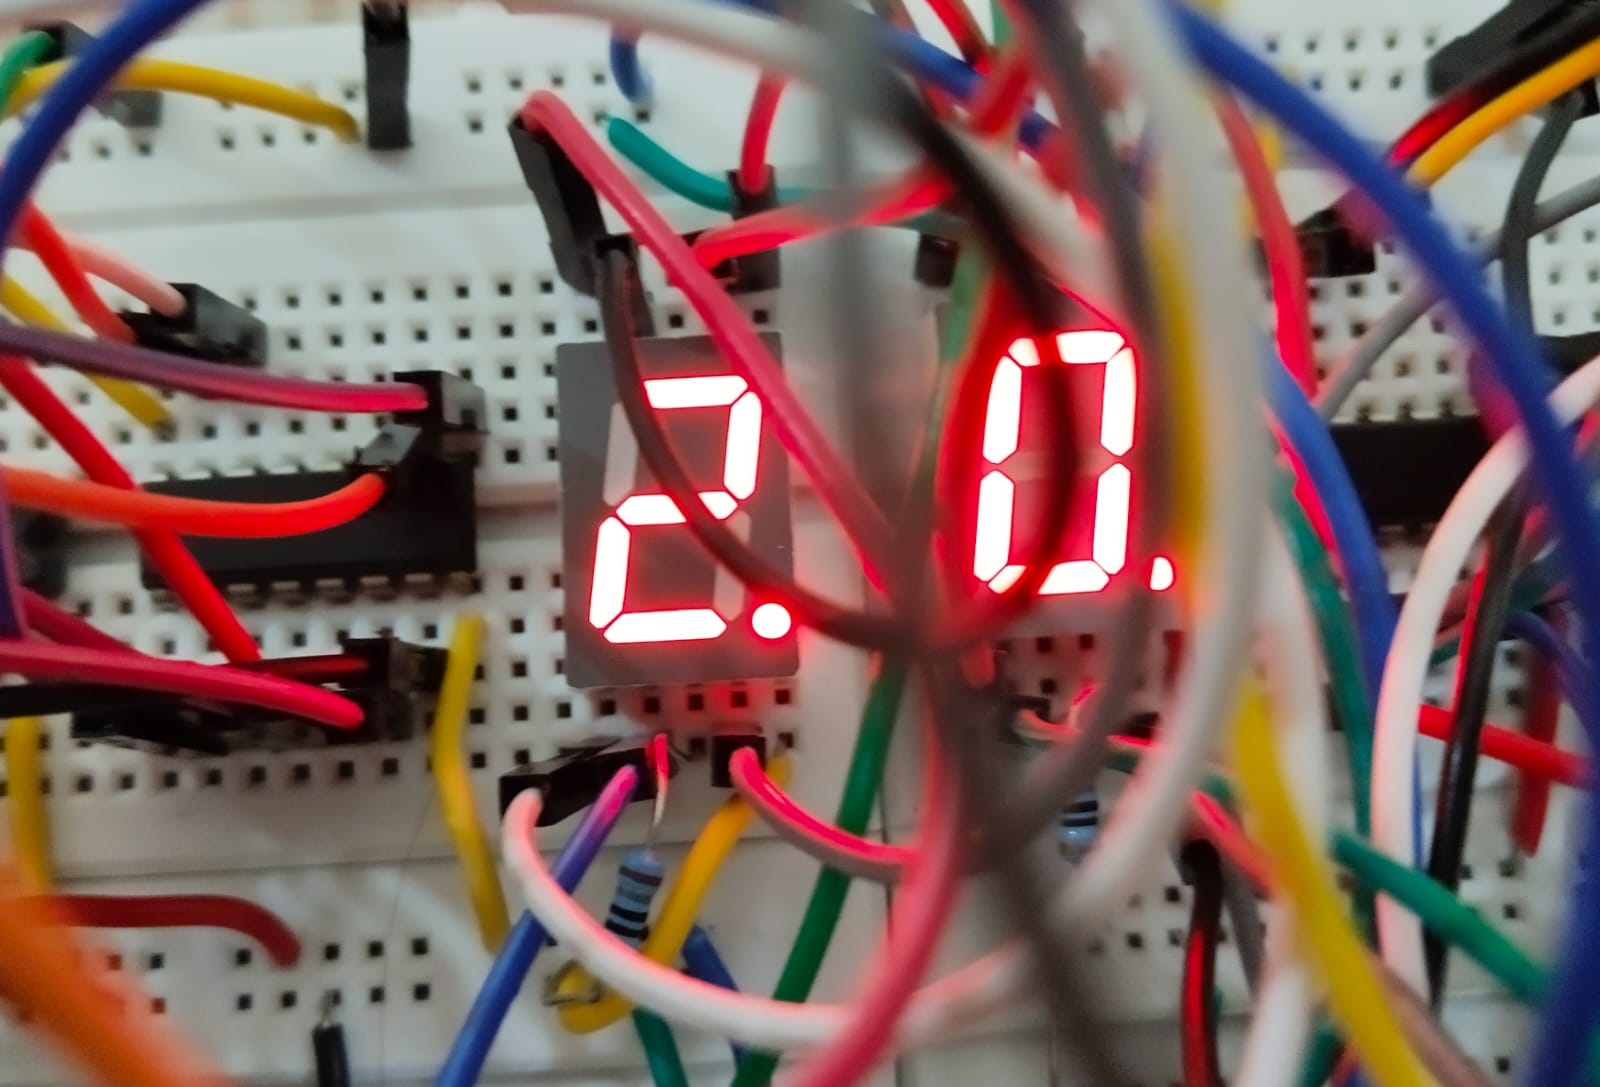
\includegraphics[width=0.6\textwidth]{figs/r_20.jpeg}
	\caption*{Circuit Displaying 20}
\end{figure}
\begin{figure}[H]
\centering
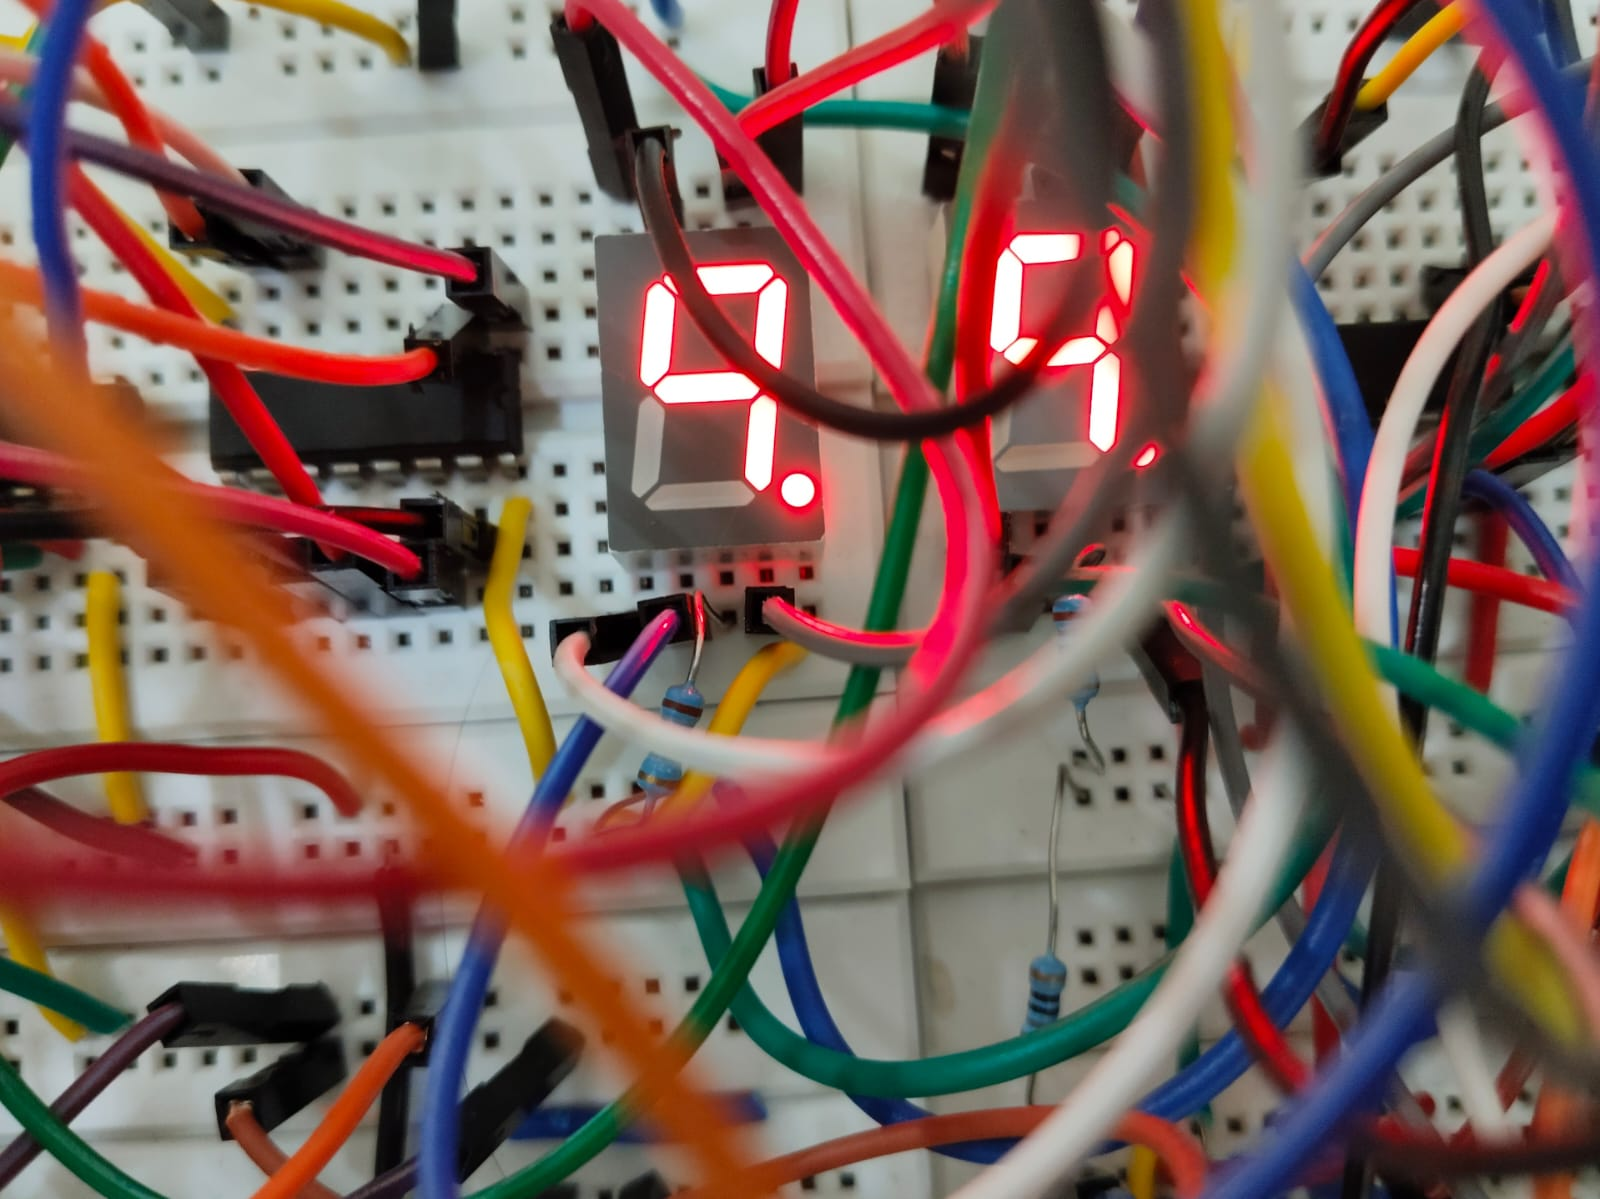
\includegraphics[width=0.6\textwidth]{figs/r_99.jpeg}
	\caption*{Circuit Displaying 99}
\end{figure}
\newpage
\subsection{\textbf{The Logic for all the connections are given below:}}
\textbf{For One's Place Digit the Logic Gates are as follows:}
\begin{figure}[H]
\centering
\resizebox{1.2\textwidth}{!}{%
\begin{circuitikz}
\tikzstyle{every node}=[font=\LARGE]
\draw (1,12.25) to[push button] (3.75,12.25);
\draw (1,7.25) to[push button] (3.75,7.25);
\node [font=\normalsize] at (0.5,12.25) {5 V};
\node [font=\normalsize] at (0.5,7.25) {5 V};
\draw (3.75,12.25) to[R] (3.75,10.5);
\draw (3.75,7.25) to[R] (3.75,5.75);
\draw (3.75,10.5) to (3.75,10.25) node[ground]{};
\draw (3.75,5.75) to (3.75,5.5) node[ground]{};
\draw (3.75,12.25) to[short] (5,12.25);
\draw (5,12.25) to[short] (5,14.75);
\draw (5,14.75) to[short] (7.5,14.75);
\draw (5,12.25) to[short] (7.5,12.25);
\draw (5,12.25) to[short] (5,9.75);
\draw (5,9.75) to[short] (7.5,9.75);
\draw (7.5,15.25) to[short] (8.5,15.25);
\draw (7.5,14.75) to[short] (8.5,14.75);
\draw (8.5,15.25) node[ieeestd and port, anchor=in 1, scale=0.89](port){} (port.out) to[short] (11.25,15);
\draw (7.5,12.75) to[short] (8.5,12.75);
\draw (7.5,12.25) to[short] (8.5,12.25);
\draw (8.5,12.75) node[ieeestd and port, anchor=in 1, scale=0.89](port){} (port.out) to[short] (11.25,12.5);
\draw (7.5,9.75) to[short] (8.5,9.75);
\draw (7.5,9.25) to[short] (8.5,9.25);
\draw (8.5,9.75) node[ieeestd and port, anchor=in 1, scale=0.89](port){} (port.out) to[short] (11.25,9.5);
\node [font=\normalsize] at (7,15.25) {$T_1(up)$};
\node [font=\normalsize] at (7,12.75) {$T_2(up)$};
\node [font=\normalsize] at (7,9.25) {$T_3(up)$};
\draw (8.75,15) to[short] (1.5,15);
\draw (8.75,9.5) to[short] (1.5,9.5);
\draw (7.5,7.25) to[short] (8.5,7.25);
\draw (7.5,6.75) to[short] (8.5,6.75);
\draw (8.5,7.25) node[ieeestd and port, anchor=in 1, scale=0.89](port){} (port.out) to[short] (11.25,7);
\draw (7.5,4.75) to[short] (8.5,4.75);
\draw (7.5,4.25) to[short] (8.5,4.25);
\draw (8.5,4.75) node[ieeestd and port, anchor=in 1, scale=0.89](port){} (port.out) to[short] (11.25,4.5);
\draw (7.5,2.25) to[short] (8.5,2.25);
\draw (7.5,1.75) to[short] (8.5,1.75);
\draw (8.5,2.25) node[ieeestd and port, anchor=in 1, scale=0.89](port){} (port.out) to[short] (11.25,2);
\draw (3.75,7.25) to[short] (7.5,7.25);
\draw (5,7.25) to[short] (5,4.75);
\draw (5,4.75) to[short] (7.5,4.75);
\draw (5,4.75) to[short] (5,2.25);
\draw (5,2.25) to[short] (7.5,2.25);
\node [font=\normalsize] at (6.75,6.75) {$T_1(down)$};
\node [font=\normalsize] at (6.75,4.25) {$T_2(down)$};
\node [font=\normalsize] at (6.75,1.75) {$T_3(down)$};
\draw (3.5,7) to[short] (1.75,7);
\draw (1.75,7.25) to[short] (1.75,2);
\draw (1.75,2) to[short] (8.75,2);
\draw (1.5,15) to[short] (1.5,9.5);
\draw (1.75,4.5) to[short] (3.75,4.5);
\draw (3,12.5) to[crossing] (7,12.5);
\draw (8.5,12.5) to[short] (8.75,12.5);
\draw (3,12.5) to[short] (1.5,12.5);
\draw (7,12.5) to[short] (8.75,12.5);
\draw (3.5,7) to[crossing] (6.5,7);
\draw (6.5,7) to[short] (8.75,7);
\draw (3.75,4.5) to[crossing] (6.25,4.5);
\draw (6.25,4.5) to[short] (8.75,4.5);
\draw (15,12.25) to[short] (16,12.25);
\draw (15,11.75) to[short] (16,11.75);
\draw (16,12.25) node[ieeestd or port, anchor=in 1, scale=0.89](port){} (port.out) to[short] (18.75,12);
\draw (15,8.5) to[short] (16,8.5);
\draw (15,8) to[short] (16,8);
\draw (16,8.5) node[ieeestd or port, anchor=in 1, scale=0.89](port){} (port.out) to[short] (18.75,8.25);
\draw (15,4.75) to[short] (16,4.75);
\draw (15,4.25) to[short] (16,4.25);
\draw (16,4.75) node[ieeestd or port, anchor=in 1, scale=0.89](port){} (port.out) to[short] (18.75,4.5);
\draw (11.25,15) to[short] (15,15);
\draw (15,15) to[short] (15,12.25);
\draw (11.25,7) to[short] (13.75,7);
\draw (13.75,7) to[short] (13.75,11.75);
\draw (13.75,11.75) to[short] (15,11.75);
\draw (11.25,12.5) to[short] (14.25,12.5);
\draw (14.25,12.5) to[crossing] (14.25,11);
\draw (14.25,11) to[short] (14.25,8.5);
\draw (14.25,8.5) to[short] (15,8.5);
\draw (11.25,4.5) to[short] (14.25,4.5);
\draw (14.25,4.5) to[short] (14.25,8);
\draw (14.25,8) to[short] (15,8);
\draw (11.25,9.5) to[short] (13,9.5);
\draw (13,9.5) to[short] (13,8.25);
\draw (13,8.25) to[crossing] (13,5.75);
\draw (15,4.75) to[crossing] (13.5,4.75);
\draw (13,5.75) to[short] (13,4.75);
\draw (13,4.75) to[short] (13.5,4.75);
\draw (11.25,2) to[short] (15,2);
\draw (15,4.25) to[short] (15,2);
\node [font=\large] at (21.5,12) {$one's digit : T_1 = J_1 = K_1$};
\node [font=\large] at (21.5,8.25) {$one's digit :T_2 = J_2 = K_2$};
\node [font=\large] at (21.5,4.5) {$one's digit :T_3 = J_3 = K_3$};
\node [font=\normalsize] at (2.5,11.75) {$Increment$};
\node [font=\normalsize] at (2.5,7.75) {$Decrement$};
\draw (0,9) to[short] (-0.5,9);
\draw (0,8.5) to[short] (-0.5,8.5);
\draw (-0.5,9) node[ieeestd or port, anchor=in 2, scale=0.89, rotate=180](port){} (port.out) to[short] (-2.75,8.75);
\draw (0,8.5) to[short] (3.75,8.5);
\draw (3.75,8.5) to[short] (3.75,7.25);
\draw (0,9) to[short] (0,13.5);
\draw (0,13.5) to[crossing] (3,13.5);
\draw (3.75,12.25) to[crossing] (3.75,12.75);
\draw (3,13.5) to[short] (3.75,13.5);
\draw (3.75,13.5) to[short] (3.75,12.75);
\node [font=\normalsize] at (-3.25,8.75) {$CLK$};
\end{circuitikz}
}%
\end{figure}

\textbf{The below Logic is for connecting the Ten's Place Digit to One's Place Digit}
\begin{figure}[H]
\centering
\resizebox{1.2\textwidth}{!}{%
\begin{circuitikz}
\tikzstyle{every node}=[font=\normalsize]
\draw (1,12.25) to[push button] (3.75,12.25);
\draw (1,7.25) to[push button] (3.75,7.25);
\node [font=\normalsize] at (0.5,12.25) {5 V};
\node [font=\normalsize] at (0.5,7.25) {5 V};
\draw (3.75,12.25) to[R] (3.75,10.5);
\draw (3.75,7.25) to[R] (3.75,5.75);
\draw (3.75,10.5) to (3.75,10.25) node[ground]{};
\draw (3.75,5.75) to (3.75,5.5) node[ground]{};
\draw (3.75,12.25) to[short] (5,12.25);
\draw (5,12.25) to[short] (5,14.75);
\draw (5,14.75) to[short] (7.5,14.75);
\draw (5,12.25) to[short] (7.5,12.25);
\draw (5,12.25) to[short] (5,9.75);
\draw (5,9.75) to[short] (7.5,9.75);
\draw (7.5,15.25) to[short] (8.5,15.25);
\draw (7.5,14.75) to[short] (8.5,14.75);
\draw (8.5,15.25) node[ieeestd and port, anchor=in 1, scale=0.89](port){} (port.out) to[short] (11.25,15);
\draw (7.5,12.75) to[short] (8.5,12.75);
\draw (7.5,12.25) to[short] (8.5,12.25);
\draw (8.5,12.75) node[ieeestd and port, anchor=in 1, scale=0.89](port){} (port.out) to[short] (11.25,12.5);
\draw (7.5,9.75) to[short] (8.5,9.75);
\draw (7.5,9.25) to[short] (8.5,9.25);
\draw (8.5,9.75) node[ieeestd and port, anchor=in 1, scale=0.89](port){} (port.out) to[short] (11.25,9.5);
\node [font=\normalsize] at (7,15.25) {$T_1(up)$};
\node [font=\normalsize] at (7,12.75) {$T_2(up)$};
\node [font=\normalsize] at (7,9.25) {$T_3(up)$};
\draw (8.75,15) to[short] (-0.5,15);
\draw (8.75,9.5) to[short] (1.5,9.5);
\draw (7.5,7.25) to[short] (8.5,7.25);
\draw (7.5,6.75) to[short] (8.5,6.75);
\draw (8.5,7.25) node[ieeestd and port, anchor=in 1, scale=0.89](port){} (port.out) to[short] (11.25,7);
\draw (7.5,4.75) to[short] (8.5,4.75);
\draw (7.5,4.25) to[short] (8.5,4.25);
\draw (8.5,4.75) node[ieeestd and port, anchor=in 1, scale=0.89](port){} (port.out) to[short] (11.25,4.5);
\draw (7.5,2.25) to[short] (8.5,2.25);
\draw (7.5,1.75) to[short] (8.5,1.75);
\draw (8.5,2.25) node[ieeestd and port, anchor=in 1, scale=0.89](port){} (port.out) to[short] (11.25,2);
\draw (3.75,7.25) to[short] (7.5,7.25);
\draw (5,7.25) to[short] (5,4.75);
\draw (5,4.75) to[short] (7.5,4.75);
\draw (5,4.75) to[short] (5,2.25);
\draw (5,2.25) to[short] (7.5,2.25);
\node [font=\normalsize] at (6.75,6.75) {$T_1(down)$};
\node [font=\normalsize] at (6.75,4.25) {$T_2(down)$};
\node [font=\normalsize] at (6.75,1.75) {$T_3(down)$};
\draw (3.5,7) to[short] (1.75,7);
\draw (1.75,2) to[short] (8.75,2);
\draw (1.75,4.5) to[short] (3.75,4.5);
\draw (3,12.5) to[crossing] (7,12.5);
\draw (8.5,12.5) to[short] (8.75,12.5);
\draw (3,12.5) to[short] (1.5,12.5);
\draw (7,12.5) to[short] (8.75,12.5);
\draw (3.5,7) to[crossing] (6.5,7);
\draw (6.5,7) to[short] (8.75,7);
\draw (3.75,4.5) to[crossing] (6.25,4.5);
\draw (6.25,4.5) to[short] (8.75,4.5);
\draw (15,12.25) to[short] (16,12.25);
\draw (15,11.75) to[short] (16,11.75);
\draw (16,12.25) node[ieeestd or port, anchor=in 1, scale=0.89](port){} (port.out) to[short] (18.75,12);
\draw (15,8.5) to[short] (16,8.5);
\draw (15,8) to[short] (16,8);
\draw (16,8.5) node[ieeestd or port, anchor=in 1, scale=0.89](port){} (port.out) to[short] (18.75,8.25);
\draw (15,4.75) to[short] (16,4.75);
\draw (15,4.25) to[short] (16,4.25);
\draw (16,4.75) node[ieeestd or port, anchor=in 1, scale=0.89](port){} (port.out) to[short] (18.75,4.5);
\draw (11.25,15) to[short] (15,15);
\draw (15,15) to[short] (15,12.25);
\draw (11.25,7) to[short] (13.75,7);
\draw (13.75,7) to[short] (13.75,11.75);
\draw (13.75,11.75) to[short] (15,11.75);
\draw (11.25,12.5) to[short] (14.25,12.5);
\draw (14.25,12.5) to[crossing] (14.25,11);
\draw (14.25,11) to[short] (14.25,8.5);
\draw (14.25,8.5) to[short] (15,8.5);
\draw (11.25,4.5) to[short] (14.25,4.5);
\draw (14.25,4.5) to[short] (14.25,8);
\draw (14.25,8) to[short] (15,8);
\draw (11.25,9.5) to[short] (13,9.5);
\draw (13,9.5) to[short] (13,8.25);
\draw (13,8.25) to[crossing] (13,5.75);
\draw (15,4.75) to[crossing] (13.5,4.75);
\draw (13,5.75) to[short] (13,4.75);
\draw (13,4.75) to[short] (13.5,4.75);
\draw (11.25,2) to[short] (15,2);
\draw (15,4.25) to[short] (15,2);
\node [font=\large] at (21.5,12) {$ten's  digit :T_1 = J_1 = K_1$};
\node [font=\large] at (21.5,8.25) {$ten's  digit :T_2 = J_2 = K_2$};
\node [font=\large] at (21.5,4.5) {$ten's  digit :T_3 = J_3 = K_3$};
\node [font=\normalsize] at (2.5,11.75) {$Increment$};
\node [font=\normalsize] at (2.5,7.75) {$Decrement$};
\draw (-8.5,13.5) to[short] (-7.5,13.5);
\draw (-8.5,13) to[short] (-7.5,13);
\draw (-7.5,13.5) node[ieeestd and port, anchor=in 1, scale=0.89](port){} (port.out) to[short] (-4.75,13.25);
\draw (-8.5,12) to[short] (-7.5,12);
\draw (-8.5,11.5) to[short] (-7.5,11.5);
\draw (-7.5,12) node[ieeestd and port, anchor=in 1, scale=0.89](port){} (port.out) to[short] (-4.75,11.75);
\draw (-4.75,12.75) to[short] (-4.5,12.75);
\draw (-4.75,12.25) to[short] (-4.5,12.25);
\draw (-4.5,12.75) node[ieeestd and port, anchor=in 1, scale=0.89](port){} (port.out) to[short] (-2.5,12.5);
\draw (-4.75,13.25) to[short] (-4.75,12.75);
\draw (-4.75,12.25) to[short] (-4.75,11.75);
\draw (-2.5,12.5) to[short] (1.5,12.5);
\draw (-0.5,15) to[short] (-0.5,12.5);
\draw (1.5,9.5) to[short] (-0.5,9.5);
\draw (-0.5,12.5) to[short] (-0.5,9.5);
\draw (-8.25,5.5) to[short] (-7.25,5.5);
\draw (-8.25,5) to[short] (-7.25,5);
\draw (-7.25,5.5) node[ieeestd and port, anchor=in 1, scale=0.89](port){} (port.out) to[short] (-4.5,5.25);
\draw (-8.25,4) to[short] (-7.25,4);
\draw (-8.25,3.5) to[short] (-7.25,3.5);
\draw (-7.25,4) node[ieeestd and port, anchor=in 1, scale=0.89](port){} (port.out) to[short] (-4.5,3.75);
\draw (-4.5,4.75) to[short] (-4.25,4.75);
\draw (-4.5,4.25) to[short] (-4.25,4.25);
\draw (-4.25,4.75) node[ieeestd and port, anchor=in 1, scale=0.89](port){} (port.out) to[short] (-2.25,4.5);
\draw (-4.5,5.25) to[short] (-4.5,4.75);
\draw (-4.5,4.25) to[short] (-4.5,3.75);
\draw (-2.25,4.5) to[short] (1.75,4.5);
\draw (1.75,7) to[short] (1.75,4.5);
\draw (1.75,4.5) to[short] (1.75,2);
\node [font=\normalsize] at (-10.5,13.5) {$ From one's digit :Q_3$};
\node [font=\normalsize] at (-8.75,13) {$\overline{Q_2}$};
\node [font=\normalsize] at (-8.75,12) {$\overline{Q_1}$};
\node [font=\normalsize] at (-8.75,11.5) {$Q_0$};
\node [font=\normalsize] at (-8.75,5.5) {$\overline{Q_3}$};
\node [font=\normalsize] at (-8.75,5) {$\overline{Q_2}$};
\node [font=\normalsize] at (-8.75,4) {$\overline{Q_1}$};
\node [font=\normalsize] at (-8.75,3.5) {$\overline{Q_0}$};
\end{circuitikz}
}%
\end{figure}

\subsection{\textbf{The Below are the Observations From the Simulation:}}
\begin{figure}[H]
\centering    
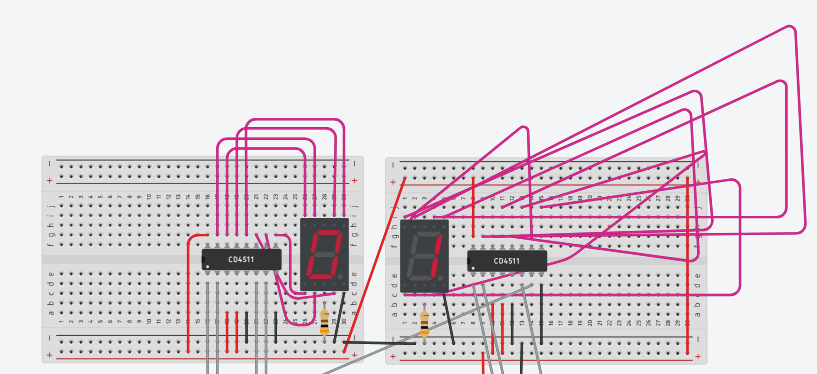
\includegraphics[width=0.5\textwidth]{figs/1.png} 
	\caption*{Displaying 1}
\end{figure}
\begin{figure}[H]
\centering    
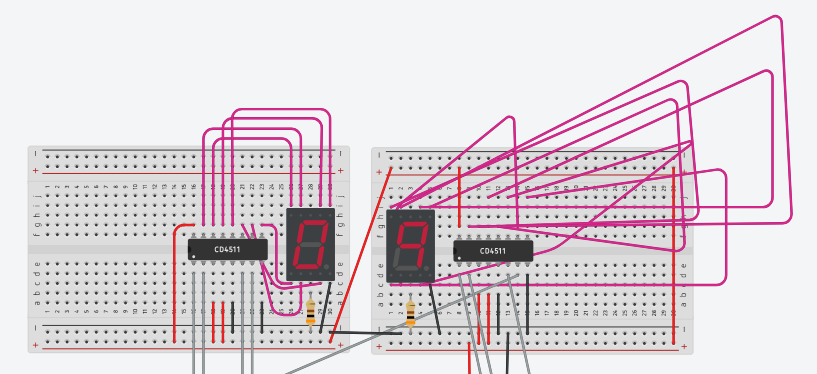
\includegraphics[width=0.5\textwidth]{figs/9.png} 
	\caption*{Displaying 9}
\end{figure}
\begin{figure}[H]
\centering    
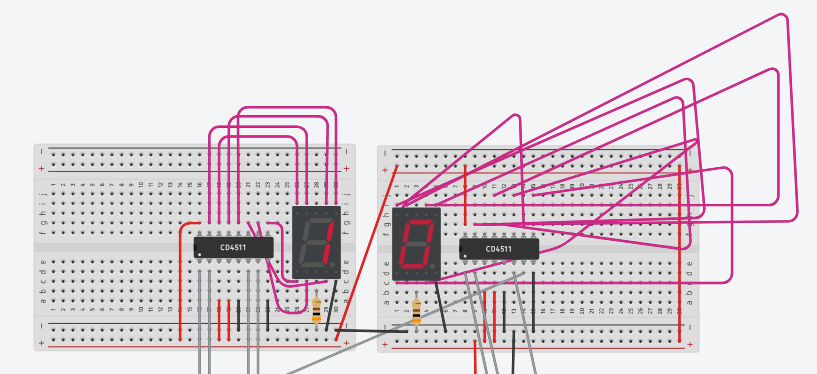
\includegraphics[width=0.5\textwidth]{figs/10.png} 
	\caption*{Displaying 10}
\end{figure}
\begin{figure}[H]
\centering    
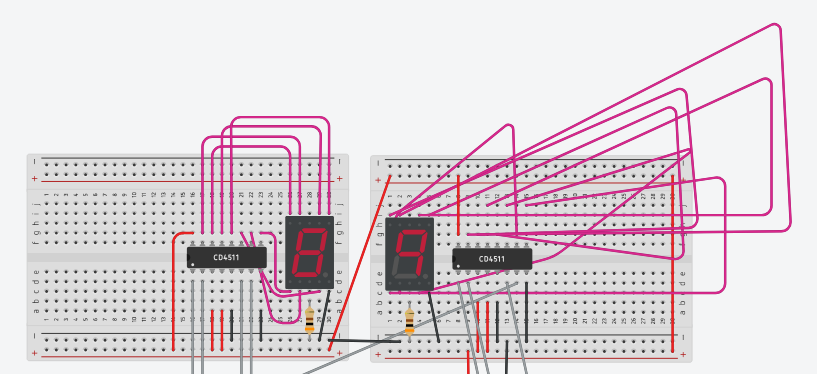
\includegraphics[width=0.5\textwidth]{figs/89.png}
	\caption*{Displaying 89}
\end{figure}
\begin{figure}[H]
\centering    
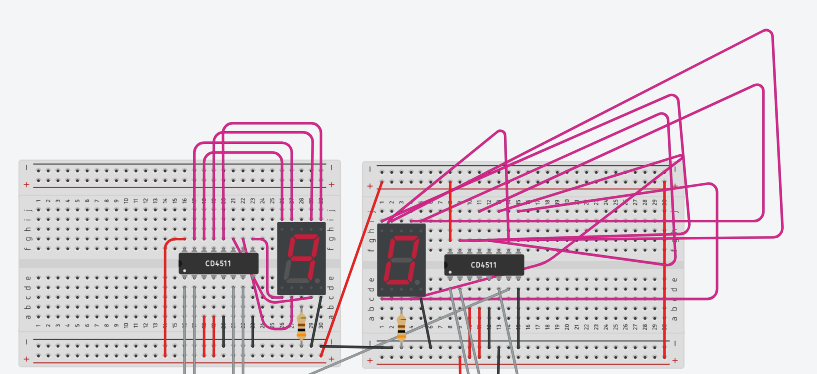
\includegraphics[width=0.5\textwidth]{figs/90.png} 
	\caption*{Displaying 90}
\end{figure}
\begin{figure}[H]
\centering    
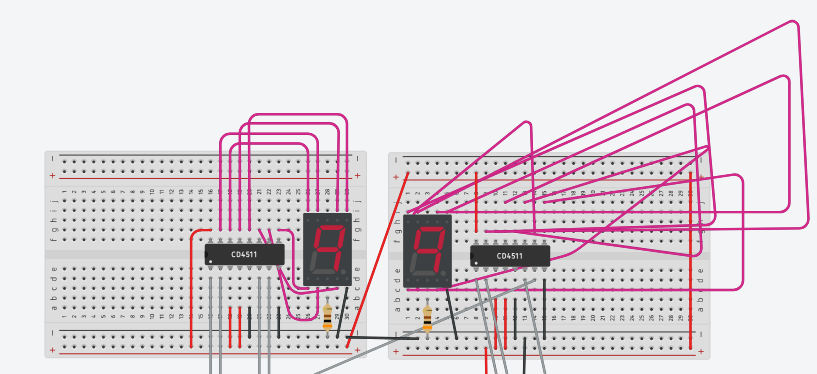
\includegraphics[width=0.5\textwidth]{figs/99.png}
	\caption*{Displaying 99}
\end{figure}

\section{Conclusion}
The up-down counter successfully demonstrates the fundamental principles of digital electronics and sequential logic. By counting in both increasing and decreasing order based on control input, it showcases how flip-flops and logic gates can be combined to perform controlled counting operations. This project not only enhances understanding of counter design but also provides practical insight into timing, synchronization, and direction control—key aspects in many digital systems. Overall, the implementation and testing of the up-down counter affirm its importance in applications such as digital clocks, memory addressing, and embedded systems.
\end{document}
